\section{Corpus study}
\label{sec:corpusstudies}

\subsection{Preliminiaries}

\subsubsection{Corpus choice}
\label{sec:gettingdata}

For the present study, I used the German \textit{Corpus from the Web} (COW) in its 2014 version DECOW14A (\citealp{SchaeferBildhauer2012full}, and \citealp{Schaefer2015b}, as well as \citealp{BiemannEa2013}, and \citealp{SchaeferBildhauer2013}, for overviews of web corpora in general and the methodology of their construction), which contains almost 21 billion tokens.%
\footnote{The COW corpora (Dutch, English, French, German, Spanish, Swedish) are made available for free at \url{https://www.webcorpora.org}.
At the time of this writing, a newer 2016 version DECOW16A has already been released.}
I chose this corpus for two main reasons.%
\footnote{The use of web data for linguistic research does require explicit and careful justification.
Due to the noisy nature and unknown composition of the web, only carefully designed and established web corpora like the COW corpora or the SketchEngine corpora \citep{KilgarriffEa2014} should be used.
Clearly, using search engine results is ``bad science'' for many reasons, most prominently total non-replicability of results, as \cite{Kilgarriff2006} pointed out more than ten years ago.
Careless use of search engine results is still found, however, see for example \citet[171--175]{DeclerckBrems2016}.}
First, the external validity of any study is increased through a higher heterogeneity of the sample \citep[30]{MaxwellDelaney2004}, and the DECOW14A corpus has clearly a much more heterogeneous composition compared to the only other very large corpus of German, the DeReKo \citep{KupietzEa2010} of the Institute for the German Language (IDS), which contains almost exclusively newspaper texts.%
\footnote{It was shown in \cite{W16-2601} that, for example, the range of topics covered is much smaller in DeReKo compared to DECOW14A.}
Second, it was already mentioned that normative grammars often adopt clear positions regarding the grammaticality of either the \NACa\ or the \PGCa.
Thus, newspaper text or any other text that conforms strongly to normative grammars might not represent the alternation phenomenon fully (and without bias) because authors and proofreaders who must adhere to normative guidelines might favour one alternative or the other explicitly.
Web corpora, on the other hand, contain at least some amount of non-standard language from forums and similar sources.
For these or similar reasons, COW corpora have been used in a number of peer-reviewed publications, for example \cite{VanGoethemHiligsmann2014}, \cite{VanGoethemHuening2015}, \cite{MuellerS2014}, \cite{Schaefer2016c}, \cite{SchaeferSayatz2014}, \cite{SchaeferSayatz2016}, and \cite{Zimmer2015}. 
Therefore, DECOW14A is a valid choice for this study.


\subsubsection{Bootstrapping pairs of lemmas}
\label{sec:bootstrappinlemmapairs}

I now turn to the sampling procedure applied to obtain concordances for manual annotation and statistical analysis.
Among the factors potentially influencing the alternation (see Section~\ref{sec:germanmeasurenps}) were lemma-specific preference effects.
Therefore, it was highly desirable to obtain a sample in which most of the highly frequent actually-occurring combinations of kind nouns and measure nouns were represented.
I applied a two-stage process in order to obtain a list of actually co-occurring measure nouns and kind nouns.
First, I generated a list of the one hundred most frequent mass nouns.
Second, I derived a list of all measure nouns with which the mass nouns co-occurred in the \NACb.

In the first step, I exported a list of all nouns in the DECOW14A01 sub-corpus sorted by their token frequency and manually went through it from the most frequent noun downwards, selecting the first one hundred mass nouns that occurred in the list.%
\footnote{DECOW14A01 is the first slice (roughly a twentieth) of the complete DECOW14A corpus.
It contains just over one billion tokens.}
Mass nouns were defined as concrete nouns which denote a substance in the broad sense, combine with uninflected mass quantifiers such as \textit{viel} `much' and \textit{wenig} `little' (\textit{viel Bier} `much beer'), and form only sortal and unit plurals (such as the plural \textit{Biere} `types of beer' or `glasses of beer').
Abstract nouns which partially behave like mass nouns (like \textit{Spaß} `fun’ or \textit{Gefahr} `danger’) were excluded because they are usually not quantified in the same way as concrete mass nouns.
The hundredth selected mass noun was \textit{Schmuck} `jewellery’, which is the 3,054th most frequent noun in the original frequency list.

This list of mass nouns was used in the second step to derive a list of measure nouns co-occurring with the mass nouns. 
In order to generate this list, I utilised the fact that a direct sequence of two nouns almost always instantiates the bare-noun NAC if the second noun is a mass noun.
I therefore searched for all sequences N\Sub{1}N\Sub{2} where N\Sub{2} was one of the mass noun lemmas extracted in in the first step.
Then, the resulting 100 lists of noun-noun combinations were each sorted by frequency in descending order and sieved manually to remove erroneous hits.
From each of the 100 lists, I also removed noun-noun combinations that had a frequency below 2, except if the individual list would have otherwise been shorter than 20 noun-noun combinations.
The result was a list of the most frequent 2,365 individual combinations of a measure noun and a mass noun.


\subsubsection{Variables and annotation}
\label{sec:variablesandannotation}

The full set of manually annotated variables for the main study is given in Table~\ref{tab:variables}.%
\footnote{All numeric variables were z-transformed (\ie\ centered to the mean and rescaled such that they have a standard deviation of 1) to facilitate their interpretation in the regression models.}
Notice first that \textit{Construction} is the response variable with the values \textit{PGCadj} and \textit{NACadj}.

\begin{table}
  \centering
  \begin{tabular}{llll}
    Unit of reference & Variable                      & Type    & Levels (for factors only) \\
    \midrule
    Document       & Badness                          & numeric &                           \\
                   & Genitives                        & numeric &                           \\
    Sentence       & Cardinal                         & factor  & Yes, No                   \\
                   & \textbf{Construction (response)} & factor  & NACadj, PGCadj            \\
                   & Measurecase                      & factor  & Nom, Acc, Dat             \\
    Kind lemma     & Kindattraction                   & numeric &                           \\
                   & (Kindcollo)                      & numeric &                           \\
                   & Kindfreq                         & numeric &                           \\
		   & Kindgender                       & factor  & MascNeut, Fem             \\
    Measure lemma  & Measureattraction                & numeric &                           \\
                   & (Measurecollo)                   & numeric &                           \\
                   & Measureclass                     & factor  & Physical, Container,      \\
                   &                                  &         & Amount, Portion, Rest     \\
                   & Measurefreq                      & numeric &                           \\
  \end{tabular}
  \caption{Annotated variables for the main study}
  \label{tab:variables}
\end{table}

The variables \textit{Kindattraction} and \textit{Measureattraction} encode the ratio with which a given kind noun lemma or measure noun lemma occurs in the \PGCd\ and the \NACb.
They were calculated from the auxiliary samples described at the end of Section~\ref{sec:gettingdata} as a log-transformed quotient.
The higher the value, the more often the noun occurs in the \PGCd\ (proportionally).
It could be argued that other measures of attraction strength could be used, for example those popularised in collostructional analysis (\citealp{StefanowitschGries2003,GriesStefanowitsch2004}; see also \citealp{Gries2015a}).
However, the goal here is to quantify how often lemmas occur in the \PGCd\ and the \NACb, and these constructions do not compete at all but are rather mutually exclusive.
While this does not preclude the use of collostructional analysis, it is an open question whether the marginals (usually called the ``expected frequencies'' in the collostructional literature), given the overall frequency of the constructions and the lemmas, are cognitively relevant in this case.
After all, the main difference between the quotient used here and the logarithmised p-values from a Fisher test is that they take these marginals into account. 
However, using collexeme strength instead of the raw frequency quotient was tried as an alternative (variables \textit{Kindcollo} and \textit{Measurecollo}); see Sections~\ref{sec:corpushierarchicalmodel} and~\ref{sec:interpretation}.
Additionally, \textit{Kindfreq} and \textit{Measurefreq} are the logarithm-transformed frequencies per 1,000,000 words of each lemma, extracted from the frequency lists distributed by the DECOW14A corpus creators on their web page.
In Section~\ref{sec:analyses}, it was hypothesised that classes of measure lemmas might have different preferences for the two alternants.
To capture this, class information was annotated for measure lemmas as \textit{Measureclass}.
The variable \textit{Cardinal} encodes whether the MNP is modified by a cardinal.

To capture the influence of style mentioned in Section~\ref{sec:analyses}, two proxy variables were used.
At the document level, the DECOW14A corpus has an annotation for \textit{Badness}.
As described in \cite{SchaeferEa2013}, \textit{Badness} measures how well the distribution of highly frequent short words in the document matches a pre-generated language model for German.
They also show that the Badness score corresponds robustly with human raters' intuitions about text coherence and text quality (see the paper for an operationalisation of this notion).
Documents with higher Badness usually contain more incoherent language, shorter sentences, etc.
If the \PGCa\ actually favours more elaborate stylistic levels, a high \textit{Badness} should be correlated with fewer occurrences.
Documents in DECOW14 have also been annotated with a variable called \textit{Genitives}.
The higher the values of this variable, the lower the proportion of genitives among all case-bearing forms is.
A high number of genitives is also indicative of a more formal, elaborate style close to the written standard.
However, the use of this variable as a regressor in the present study might be considered problematic.
Since the \PGCa\ contains a genitive itself, the regressor variable \textit{Genitive} and the document-level variable \textit{Genitives} are not fully independent.
Since instances of the \PGCa\ make up for only a minute fraction of all genitives, however, I still use \textit{Genitives} as a regressor.%
\footnote{A reviewer suggested that a fully fledged multidimensional analysis \citep{Biber1988} would help to improve the operationalisation of the influence of style.
This sounds plausible, but there simply is no large corpus of German for which similar data have been published.
In the meantime, the creators of COW and the Institut für Deutsche Sprache (IDS) Mannheim have developed a similar annotation framework (COReX), and the COW creators have pre-released a non-public beta version of the corresponding data base for DECOW16A to their users.
This data base contains 118 automatically extracted lexico-grammatical features for each document.
However, at this time, it is not recommended for use in published research.
Also, the genitive is generally considered a good indicator of style in German, and its frequency is usually high enough such that the \textit{Genitives} score is a stable measure even for shorter documents (compared to first or second person pronouns, for example, which are totally absent in a majority of documents).
The genitive is still the dominant attributive case in German.}

Finally, two variables were added as nuisance variables in the context of the present study.
First, it was reported in the literature that MNPs in the dative and with a masculine or neuter kind noun favour the \PGCa\ more than the corresponding nominative and accusative MNPs \citep{Hentschel1993,Zimmer2015}.
As an example, \textit{mit einem Stück frischen Brots} `with a piece of fresh bread' (\PGCa) would be preferred more strongly against \textit{mit einem Stück frischem Brot} (\NACa).
As with all the examples, native speakers of German will most likely notice that differences are subtle.
To control for this effect, the case of the measure noun was manually annotated (variable \textit{Measurecase}).
Second, due to differences in case syncretisms, it is possible that feminine kind nouns have slightly different preferences than masculine and neuter ones, and the appropriate variable \textit{Kindgender} was annotated.

\subsection{Pre-study: main prototype effects in the non-alternating constructions}

The main study to be reported below deals exclusively with the alternating constructions, as is customary in alternation modelling.
However, the prototypical features described in Section~\ref{sec:prototypeeffects} should be observable in the non-alternating cases as well if the theory laid out in Section~\ref{sec:analyses} is correct.
Therefore, in this section I examine the distribution of the prototypical features in the non-alternating cases to see whether they are in accord with the theoretical predictions.

For this pre-study, each of the 2,365 combinations of measure noun lemma and kind noun lemma were queried in the \NACb\ and the \PGCd.
Each of the resulting 2,365 concordances was scaled down randomly to a size of maximally 100 sentences, and from the resulting 35,766 sentences, 5,000 were randomly sampled for the statistical analysis.
All features described in Section~\ref{sec:variablesandannotation} were annotated except for the ones which do not apply in the non-alternating case (\textit{Kindattraction}, \textit{Measureattraction}, and \textit{Measurecase}).
The aggregated counts for each concordance were analysed in the form of a multilevel logistic regression model using R \citep{R} and the \textit{lme4} package \citep{Bates2010,BatesEa2015}.%
\footnote{An alternative \textit{BOBYQA} optimiser from the \textit{nloptr} package \citep{Johnson2017} was used for all fits with \textit{lme4} reported in this paper.}

\begin{table}
  \centering
  \resizebox{\textwidth}{!}{
    \begin{tabular}{llrlrrrc}
    Model level  & Regressor         & $\text{p}_{\text{PB}}$ & Factor level & Coefficient & CI low & CI high & CI excludes 0 \\
    \midrule
    First        & Badness           &                 &              &       &  &   &              \\
                 & Cardinal          &                 & No           &       &  &   &              \\
                 & Genitives         &                 &              &       &  &   &              \\
    
    Second       & (Kindfreq)        &                 &              &       &  &   &              \\
    (Kind)       & (Kindgender)      &                 &              &       &  &   &              \\[0.5\baselineskip]
    
    Second       & Measureclass      &                 & Container    &       &  &   &              \\
    (Measure)    &                   &                 & Rest         &       &  &   &              \\
                 &                   &                 & Amount       &       &  &   &              \\
                 &                   &                 & Portion      &       &  &   &              \\
                 & (Measurefreq)     &                 &              &       &  &   &              \\

  \end{tabular}
  }
  \caption{Coefficient table with 95\% bootstrap confidence intervals for the pre-study; the intercept is XXX}
  \label{tab:smalltable}
\end{table}

The coefficient estimates are specified in Table~\ref{tab:smalltable} for each regressor (or regressor level) in the columns labelled \textit{Coefficient}.
Given the coding of the response variable, coefficients leaning to the positive side can be interpreted as describing a context typical of the \PGCd.
For a robust quantification of the precision of the estimation, I ran a parametric bootstrap (using the \mbox{\textit{confint.merMod}} function from \textit{lme4}) with 1,000 replications and using the percentile method for the calculation of the intervals.
The resulting 95\% bootstrap confidence intervals are reported in Table~\ref{tab:smalltable} in the columns labelled \textit{CI low} and \textit{CI high} (= upper and lower 2.5th percentiles).
The column \textit{CI excludes 0} shows an asterisk for those intervals that do not include 0.
Furthermore, for each regressor, a p-value was obtained by dropping the regressor from the full model, re-estimating the nested model, and comparing it to the full model.
Instead of inexact Wald approximations and Likelihood Ratio Tests, I used a drop-in bootstrap replacement for the Likelihood Ratio Test from the function \textit{PBmodcomp} from the \textit{pbkrtest} package \citep{HalekohHojsgaard2014}.
I call the corresponding value $p_{\text{PB}}$, and it is given in the respective columns in Table~\ref{tab:smalltable}.
Regressors which did not reach sig=0.05 in pbkrtest (\textit{Kindfreq}, \textit{Kindgender}, and \textit{Measurefreq}) were removed from the model, appear in brackets in Table~\ref{tab:smalltable}, and have no coefficient estimates.



\subsection{Main study: the alternation}
\label{sec:annotation}
\label{sec:corpushierarchicalmodel}

For the main study, each of the 2,365 noun–noun combinations was queried in the alternating constructions \PGCa\ and \NACa\ in DECOW14A.%
\footnote{Due to processing considerations with the COW interface at the time, only ten slices of DECOW14A were used, which add up to approximately 10 billion tokens.}
For the manual annotation process, a random sub-sample was generated.
For each mass noun, the concordance was downsampled randomly to maximally 100 sentences, which resulted in 6,843 sentences without further downsampling.
In the manual annotation process the size was further reduced to 5,063 sentences due to removal of noisy material, erroneous hits, and uninformative cases where the measure noun was in the genitive, in which case the \NACa\ cannot be distinguished from the \PGCa.
Given the careful sampling procedure described in this section, we can be highly certain that it contains all relevant and reasonably frequent noun–noun combinations in the target constructions.%
\footnote{In a similar fashion, the 100 most frequent measure nouns occurring with plural kind nouns were listed and queried, resulting in a sample of 871 sentences.
As stated in Section~\ref{sec:germanmeasurenps}, the \NACa\ is virtually never used with plural kind nouns, and this sample was not used except for quantifying the frequency of occurrence of the constructions (67 times \NACa\ and 794 times \PGCa).
The sample is distributed with the data package accompanying this paper.}

Finally, two auxiliary samples were also drawn.
As mentioned in Section~\ref{sec:analyses}, the distribution of the measure noun and kind noun lemmas in the \NACb\ and the \PGCd\ with a determiner will be modelled as factors influencing the alternation.
Therefore, all noun-noun pairs from the process described above were also queried in the two non-alternating constructions, resulting in 17,252 hits for the \PGCd\ and 315,635 hits for the \NACb.

\begin{figure}[hb!]
  \centering
  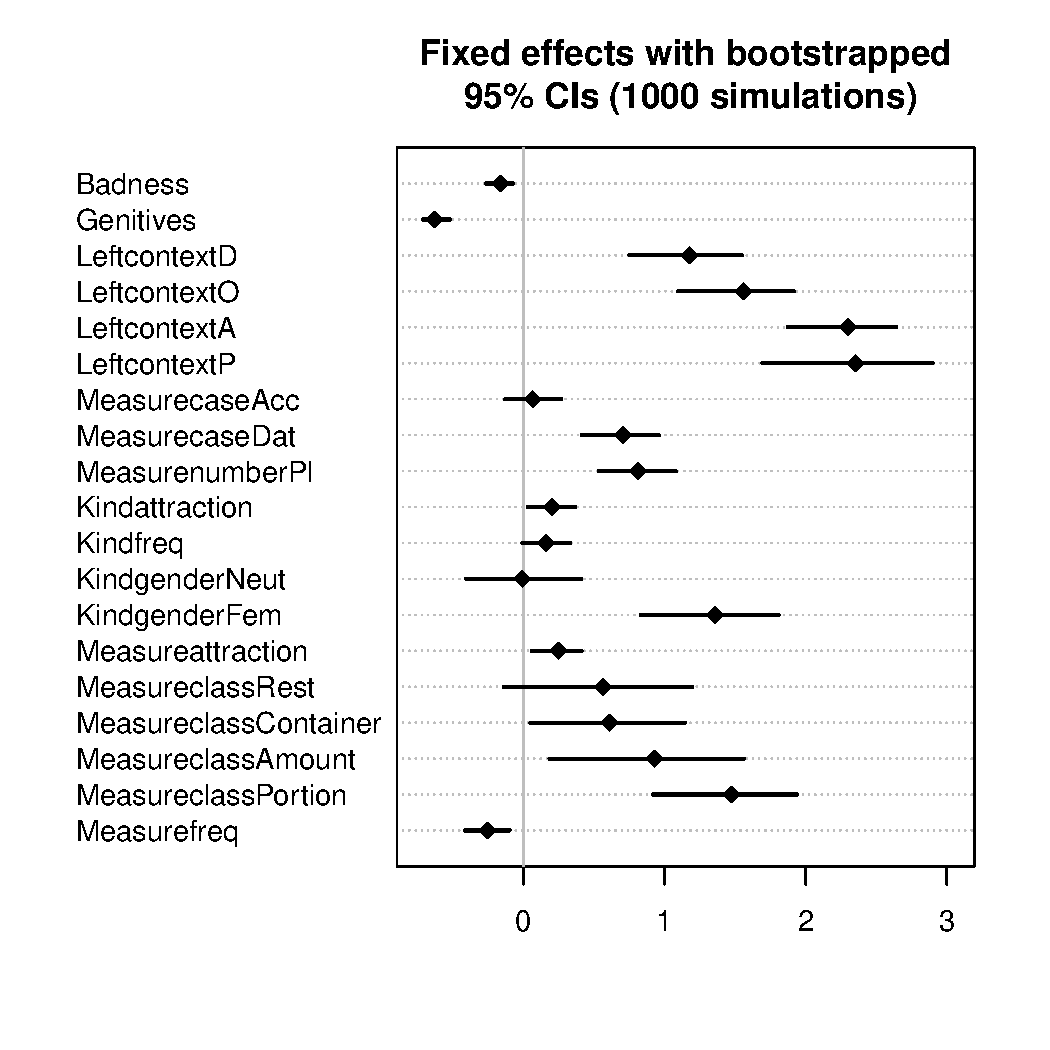
\includegraphics[width=0.85\textwidth]{../R/output/corpus_fixeffs}
  \caption{Coefficients with 95\% confidence intervals (for details see text); the intercept is -4.328}
  \label{fig:fixeffs}
\end{figure}

Then, a multilevel logistic regression model was fit which models the influence of the regressors specified in Table~\ref{tab:variables} on the probability that the \PGCa\ is chosen over the \NACa.
All regressors from Table~\ref{tab:variables} were included, and the measure lemma and the kind noun lemma were specified as varying-intercept random effects.
The sample size was \textit{n=}5,063 with 1,134 cases of \PGCa\ and 3,929 cases of \NACa.
The results of the estimation are shown in Table~\ref{tab:bigtable} and in Figure~\ref{fig:fixeffs}.
The intercept comprises \textit{Cardinal=Yes}, \textit{Measurecase=Nom}, \textit{Kindgender=Masc}, \textit{Measureclass=Physical}, and 0 for all numeric z-transformed regressors.
It was estimated at -4.328.

The regressors with the measure lemma as their unit of reference have no within-measure lemma variance, and the \textit{glmer} function automatically estimates them as \textit{group level predictors} (or \textit{second-level effects}), cf.\ \citet[265--269,302--304]{GelmanHill2006} and Section~\ref{sec:itemandexemplareffects}.
The same goes for those listed with the kind lemma as their unit of reference.
Given the coding of the response variable, coefficients leaning to the positive side can be interpreted as favouring the \PGCa.

\begin{table}
  \centering
  \resizebox{\textwidth}{!}{
    \begin{tabular}{llrlrrrc}
    Model level  & Regressor         & $\text{p}_{\text{PB}}$ & Factor level & Coefficient & CI low & CI high & CI excludes 0 \\
    \midrule
    First        & Badness           &  0.002                 &              & -0.152      & -0.247 & -0.061  & *             \\
                 & Cardinal          &  0.001                 & No           &  1.189      &  0.862 &  1.466  & *             \\
                 & Genitives         &  0.001                 &              & -0.693      & -0.768 & -0.592  & *             \\
                 & Measurecase       &  0.001                 & Acc          &  0.030      & -0.150 &  0.212  &               \\
                 &                   &                        & Dat          &  0.705      &  0.455 &  0.944  & *             \\[0.5\baselineskip]
    
    Second       & Kindattraction    &  0.020                 &              &  0.225      &  0.049 &  0.393  & *             \\
    (Kind)       & Kindfreq          &  0.095                 &              &  0.146      & -0.023 &  0.301  &               \\
                 & Kindgender        &  0.001                 & Neut         &  0.021      & -0.367 &  0.392  &               \\
                 &                   &                        & Fem          &  1.269      &  0.800 &  1.709  & *             \\[0.5\baselineskip]
    
    Second       & Measureattraction &  0.001                 &              &  0.282      &  0.106 &  0.447  & *             \\
    (Measure)    & Measureclass      &  0.001                 & Container    &  0.252      & -0.265 &  0.788  &               \\
                 &                   &                        & Rest         &  0.421      & -0.209 &  1.063  &               \\
                 &                   &                        & Amount       &  0.831      &  0.215 &  1.432  & *             \\
                 &                   &                        & Portion      &  1.217      &  0.675 &  1.684  & *             \\
                 & Measurefreq       &  0.005                 &              & -0.231      & -0.363 & -0.079  & *             \\

  \end{tabular}
  }
  \caption{Coefficient table with 95\% bootstrap confidence intervals for the main study; the intercept is -4.328}
  \label{tab:bigtable}
\end{table}

Standard diagnostics show that the model quality is quite good.%
\footnote{Notice that no aggressive model selection was applied, especially not upward model selection including probing for interactions.
I am convinced that the model should be specified based on theoretical considerations (and known nuisance effects) to avoid the dangers of data dredging and to avoid models which are difficult to interpret.
Removal of useless regressors (judging by, for example, the pbkrtest and coefficients of determination) is the only type of model selection I allow in my research.}
Nakagawa \& Schielzeth's pseudo-coefficient of determination is $R_m^2=0.409$ and $R^2_c=0.495$ (see \citealp{Gries2015} for a basic introduction to these $R^2$ measures, or else \citealp{NakagawaSchielzeth2013}).
The rate of correct predictions is 0.843, which means a proportional reduction of error of $\lambda=0.297$.
Generalised variance inflation factors for the regressors were calculated to check for multicollinearity \citep{FoxMonette1992,ZuurEa2010}, and none of the corrected $\text{GVIF}^{1/2\text{df}}$ was higher than 1.6.
The lemma intercepts have standard deviations of $\sigma_{\text{Measurelemma}}=0.448$ and $\sigma_{\text{Kindlemma}}=0.604$.
Only \textit{Kindfreq} ($\mpPB=0.095$) can be seen as slightly too high to be convincing, failing at sig=0.05.

Using collexeme strength (\textit{Measurecollo} and \textit{Kindcollo}) instead of the quotient for the attraction strength (\textit{Measureattraction} and \textit{Kindattraction}) was not successful.
While the attraction measures reach satisfying sig levels, the $\text{p}_{\text{PB}}$ value for \textit{Kindcollo} was 0.191 and the one for \textit{Measurecollo} was 0.443.
The coefficients of determination drop to $R_m^2=0.383$ and $R^2_c=0.490$.


\subsection{Interpretation}
\label{sec:interpretation}


%\hl{As collostructional analysis is relatively popular in some cognitively oriented areas of corpus linguistics, I tried using collexeme strength as a regressor (with smoothing to remedy the mathematical problems), and the results were unsatisfactory compared to the simple quotient used here.
%The corresponding regressor did not even reach sig=0.1 in the pbkrtest.
%Both the cognitive underpinnings and the math behind collostructional analysis are still much debated (see prominently \citealp{SchmidKuechenhoff2013,KuechenhoffSchmid2015}), I see this result }


% ATTRACTION

\begin{figure}[h!]
  \centering
  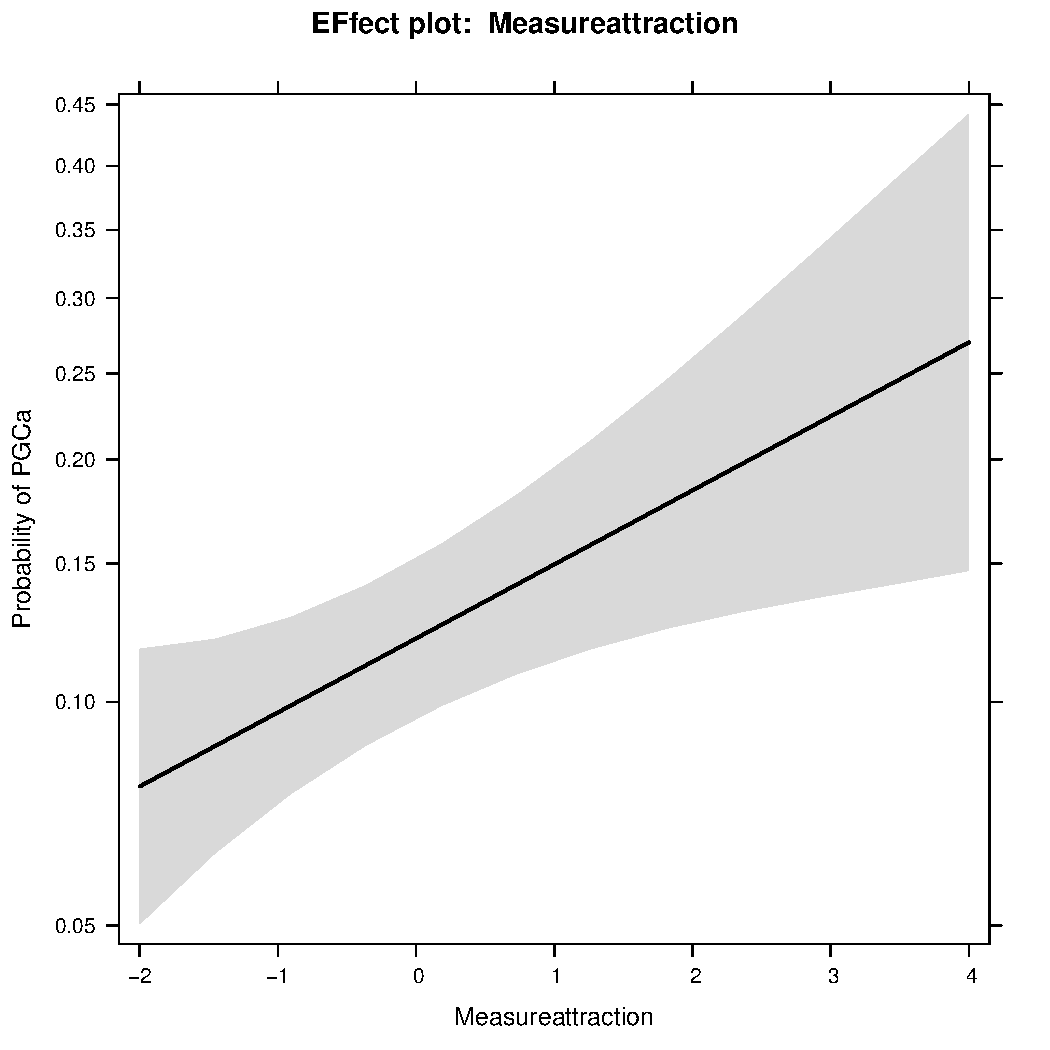
\includegraphics[width=0.5\textwidth]{../R/output/corpus_Measureattraction}~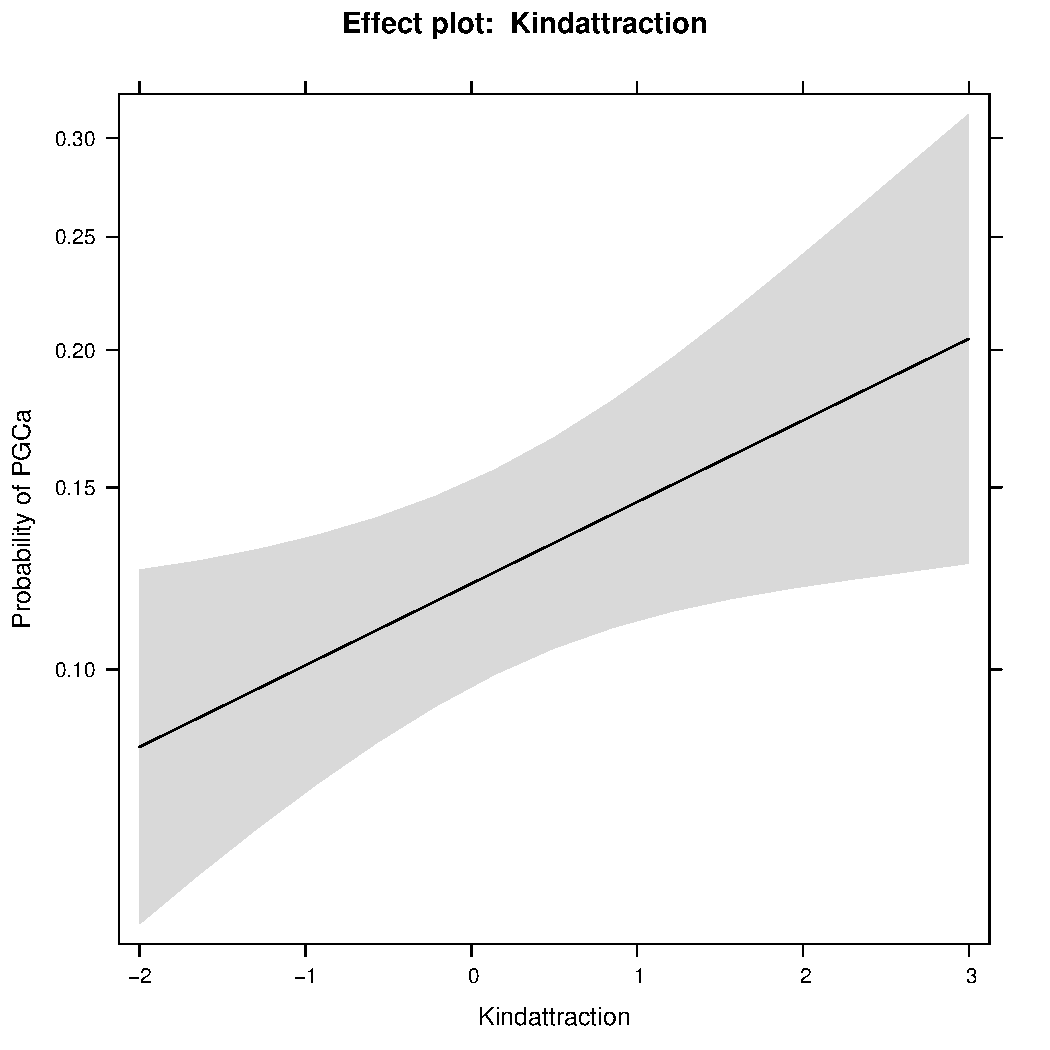
\includegraphics[width=0.5\textwidth]{../R/output/corpus_Kindattraction}
  \caption{Effect plots for the regressors \textit{Measureattraction} and \textit{Kindattraction}; y-axes are not aligned}
  \label{fig:eff:attraction}
\end{figure}

The results reported in Section~\ref{sec:corpushierarchicalmodel} generally confirm the hypotheses from Section~\ref{sec:analyses}.
First, the prototypicality effect related to the non-alternating \PGCd\ and \NACb\ can be shown (see the effect plots in Figure~\ref{fig:eff:attraction}).%
\footnote{Effect plots were created using the \textit{effects} package \citep{Fox2003}.
They show the changes in probability for the outcome (y-axis) dependent on values of a regressor (x-axis) at typical values of all other regressors.
The vertical bars (categorical variables), and the grey areas (continuous variables) are asymptotic 95\% confidence intervals calculated from \textit{glmer}.
They are not bootstrapped.
Readers should be aware that the axes are specifically scaled so as to result in a linear plot, and that the range of the axes varies between plots.}
The effect is as expected:
if a lemma appears relatively more often in the \PGCd\ (compared to its frequency in the \NACb), the \PGCa\ tends to be chosen over the \NACa\ with this specific lemma.
The effect for measure nouns is stronger, and it was estimated with higher precision.

An interesting picture emerges for the lemma frequencies.
A higher-than-average lemma frequency of measure nouns favours the \NACa\ ($\beta_{\text{Measurefreq}}=-0.231$, $\mpPB=0.005$), which is as expected if we assume at least a tendency for highly grammaticalised items to be more frequent.
With kind nouns, higher frequency seems to favour the \PGCa ($\beta_{\text{Kindfreq}}=0.146$, $\mpPB=0.095$).
However, there is no clear theoretical interpretation (see Section~\ref{sec:analyses}), and the estimate is imprecise (not significant at $\alpha=0.05$, see above).
The effect can therefore be ignored or treated as a nuisance variable.


% GRAMMATICALISATION
% => lemmas and lemma classes

\begin{figure}[h!]
  \centering
  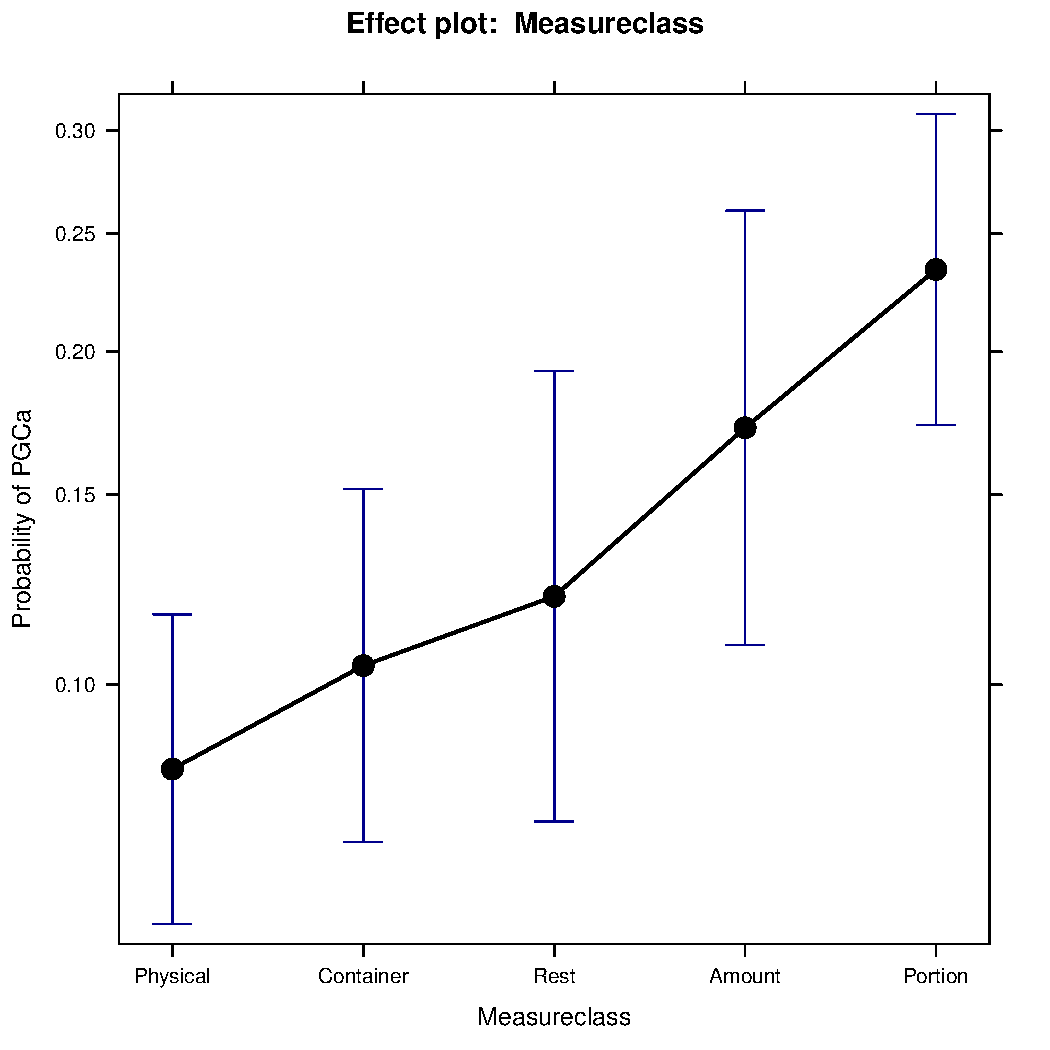
\includegraphics[width=0.5\textwidth]{../R/output/corpus_Measureclass}
  \caption{Effect plot for the regressor \textit{Measureclass}}
  \label{fig:eff:measureattraction}
\end{figure}

In Section~\ref{sec:analyses}, it was also hypothesised that classes of measure nouns with a higher degree of grammaticalisation should favour the \NACa.
The \textit{Measureclass} second-level predictor was successfully estimated ($\mpPB=0.001$).
Looking at the effect plot in Figure~\ref{fig:eff:measureattraction}, it is evident that abstract non-referential physical measure nouns (such as \textit{Gramm} `gram' or \textit{Liter} `litre') with a high degree of grammaticalisation favour the \NACa.
At the other end of the scale, nouns denoting natural portions like \textit{Haufen} `heap', \textit{Bündel} `bundle', \textit{Schluck} `gulp' favour the \PGCa.
These are referential nouns, confirming the hypothesis that it is prototypical of the PGC to contain two referential nouns, while the NAC prototypically only contains one (the kind noun).

% CARDINALS

\begin{figure}[h!]
  \centering
  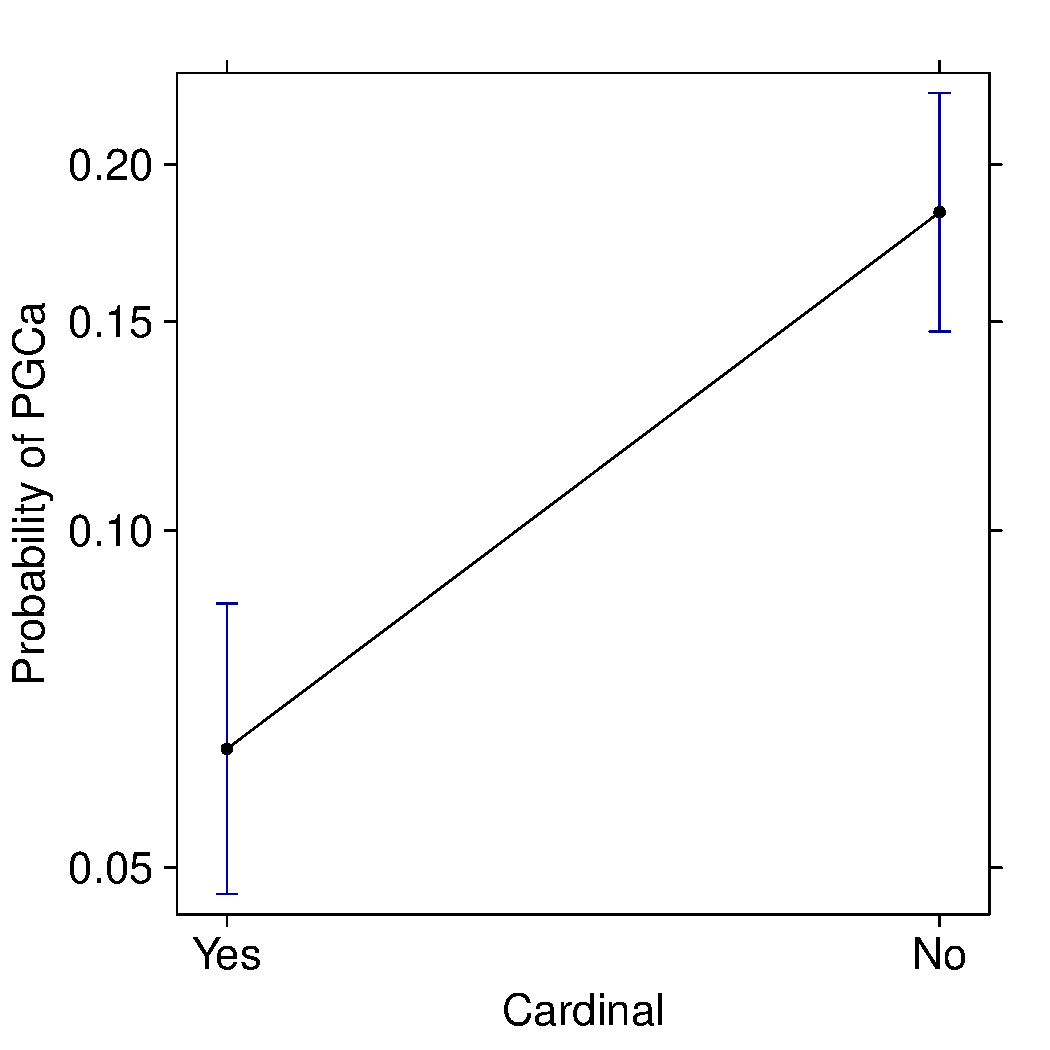
\includegraphics[width=0.5\textwidth]{../R/output/corpus_Cardinal}
  \caption{Effect plot for the regressor \textit{Cardinal}}
  \label{fig:eff:leftcontext}
\end{figure}

I now turn to the predicted effect of cardinals as modifiers of the measure noun.
Figure~\ref{fig:eff:leftcontext} shows that cardinals indeed influence the choice of the alternant ($\mpPB=0.001$), and that cardinals have a strong tendency to co-occur with the \NACa.
This effect was predicted in Section~\ref{sec:analyses}.

% REGISTER
% => Badness
% => Genitives

The style-related proxy variables point in the expected direction.
Increased \textit{Badness} of the document favours the \NACa\ ($\beta_{\text{Badness}}=-0.152$, $\mpPB=0.002$), and so does a lower density of genitives ($\beta=-0.693$, $\mpPB=0.001$).
While these are merely proxies to style (and partially circular in the case of \textit{Genitives}), this result can at least encourage future work into stylistic effects. 

% NUISANCE
% => dative effect
% => frequency

The influence of \textit{Measurecase} ($\mpPB=0.001$) is as predicted in previous analyses (see Section~\ref{sec:analyses}).
A measure noun in the dative favours the \PGCa\ with $\beta_{\text{MeasurecaseDat}}=0.705$ (compared to the nominative, which is on the intercept).
Although \textit{Measurecase} is a nuisance variable in the context of this study, convergence with previous work strengthens its validity.

